\documentclass[conference]{IEEEtran}
\IEEEoverridecommandlockouts
\usepackage{cite}
\usepackage{amsmath,amssymb,amsfonts}
\usepackage{algorithmic}
\usepackage{graphicx}
\usepackage{textcomp}
\usepackage{xcolor}
\usepackage{booktabs}
\usepackage{url}
\def\BibTeX{{\rm B\kern-.05em{\sc i\kern-.025em b}\kern-.08em
    T\kern-.1667em\lower.7ex\hbox{E}\kern-.125emX}}

\begin{document}

\title{BanglaVision60K: A Large-Scale Diverse Bengali Image Captioning Dataset}


\maketitle

\begin{abstract}
The rapid advancement of Vision-Language Models (VLMs) has been predominantly restricted to English, driven by the availability of massive, high-quality multimodal datasets. In contrast, regional and low-resource languages such as Bengali despite being one of the most widely spoken languages globally severely lack large-scale, culturally aligned multimodal corpora. This scarcity fundamentally hinders the development of generative multimodal AI tailored for South Asian demographics. To bridge this critical gap, we introduce \textbf{BanglaVision60K}, a highly comprehensive, linguistically diverse, and culturally nuanced Bengali Image Captioning dataset. The dataset comprises precisely 60,000 unique images meticulously curated from globally recognized repositories (MS COCO and Flickr30k) as well as regional sources (BNATURE), ensuring a robust variance in visual semantics. Each image is paired with 5 distinct Bengali captions, culminating in a total of 300,005 high-quality descriptive annotations. The captions were generated through a rigorous three-stage hybrid annotation pipeline involving manual human translation, AI-enhanced contextual generation utilizing the Qwen Large Vision-Language Model, and stringent human-in-the-loop manual cleaning. Extensive Exploratory Data Analysis (EDA) reveals a rich linguistic diversity with a vocabulary size of 46,499 unique tokens, a Zipfian cumulative coverage distribution, and an average length of 9.53 words per caption. We establish a robust standardized train-validation-test split (80-10-10) and propose comprehensive baseline benchmarking protocols using modern Vision-Encoder-Decoder architectures. BanglaVision60K provides a foundational resource for training, fine-tuning, and evaluating state-of-the-art multimodal AI models for the Bengali language.
\end{abstract}

\begin{IEEEkeywords}
Image Captioning, Vision-Language Models (VLM), Bengali NLP, Multimodal Dataset, Deep Learning, Vision Transformers (ViT)
\end{IEEEkeywords}

\section{Introduction}
Image captioning, the task of automatically generating accurate and contextually relevant textual descriptions for visual inputs, stands as a fundamental challenge at the intersection of Computer Vision (CV) and Natural Language Processing (NLP). In recent years, Transformer-based Vision-Language models (VLMs) have achieved unprecedented success in this domain \cite{li2023blip2, liu2023llava, bai2023qwenvl}. Models such as BLIP-2 \cite{li2023blip2}, InstructBLIP \cite{dai2023instructblip}, and LLaVA \cite{liu2023llava} have demonstrated remarkable zero-shot capabilities and visual reasoning skills. However, the vast majority of these architectural and empirical advancements are heavily tailored for the English language \cite{chen2024paligemma, radford2023clip}. This success is almost entirely predicated on the existence of massive, high-quality, human-annotated datasets like MS COCO \cite{lin2014microsoft}, Flickr30k \cite{young2014image}, and Conceptual Captions.

For Bengali, which ranks as one of the most spoken languages globally with nearly 300 million native speakers, the progress in multimodal artificial intelligence has been severely hindered by a critical bottleneck: the scarcity of high-quality, large-scale, and culturally aligned annotated datasets \cite{hossain2023bengali, rahman2024vision}. Bengali is a morphologically rich, highly inflected language with complex syntactic structures that do not easily map one-to-one with English \cite{chowdhury2023survey}. Existing Bengali image captioning datasets are either too small to effectively train modern deep learning architectures from scratch or rely heavily on crude, automated machine translations that lack cultural context, contextual nuance, and linguistic diversity required for natural language generation \cite{das2023captioning, sarker2024data}.

To address this glaring disparity and catalyze regional research in multimodal AI, we present \textbf{BanglaVision60K}, a large-scale, high-quality dataset containing exactly 60,000 images paired with 300,005 linguistically rich Bengali captions. 

The core contributions of our research are outlined as follows:
\begin{itemize}
    \item \textbf{Large-Scale Cultural Dataset}: Recognizing the severe lack of large-scale culturally aligned Bengali datasets, we developed BanglaVision60K, a highly curated dataset containing 60,000 diverse cultural images.
    \item \textbf{Linguistic Diversity}: We introduced robust linguistic diversity by providing exactly 5 distinct caption variations per image, ensuring the models learn various semantic and structural perspectives.
    \item \textbf{High-Quality Annotation}: We employed a meticulous re-captioning and hybrid annotation pipeline combining Qwen-VL's contextual generation with rigorous human-in-the-loop filtering to guarantee unprecedented caption quality.
    \item \textbf{Baseline Benchmarking}: We present a robust standardized evaluation protocol and provide extensive matrix data (BLEU, METEOR, CIDEr) to demonstrate that models trained on our dataset achieve superior performance on culturally contextualized Bengali images.
\end{itemize}

\section{Related Work}
\subsection{Vision-Language Foundation Models}
The paradigm of Vision-Language representation learning has shifted dramatically from early CNN-RNN encoder-decoder networks to large-scale Transformer-based foundation models. CLIP \cite{radford2023clip} revolutionized the field by aligning images and text in a shared latent space via contrastive learning. Subsequent architectures like BLIP-2 \cite{li2023blip2} and InstructBLIP \cite{dai2023instructblip} introduced Q-Former structures to bridge frozen image encoders with large language models, enabling state-of-the-art image captioning with minimal fine-tuning. Recent advancements like Qwen-VL \cite{bai2023qwenvl} and LLaVA \cite{liu2023llava} utilize massive scale instruction-tuning to perform complex visual reasoning. However, these models inherently exhibit a strong English bias, heavily underperforming in zero-shot tasks for low-resource languages like Bengali \cite{mahmud2025qwen}.

\subsection{Large-Scale Image Captioning Datasets}
The success of the aforementioned models relies entirely on datasets like MS COCO \cite{lin2014microsoft}, which contains 330K images with 1.5 million captions, and Flickr30k \cite{young2014image}, focusing on human actions. While attempts have been made to automatically translate these datasets using Google Translate or similar APIs \cite{karim2025evaluating}, such translations often suffer from "translationese" artifacts, loss of idioms, and incorrect grammatical structures, making them suboptimal for training native-sounding generative models \cite{sarker2024data}.

\subsection{Bengali NLP and Multimodal Resources}
In the realm of Bengali NLP, significant strides have been made in text-only tasks with the introduction of monolingual corpora like BanglaLM and various transformer-based language models (e.g., BanglaBERT). However, multimodal resources remain scarce \cite{hossain2023bengali}. Early attempts at Bengali image captioning \cite{das2023captioning} relied on very small datasets (under 10,000 images) constrained to specific domains. Recent efforts \cite{ahmed2024multimodal, khatun2024benchmarking} have highlighted the urgent need for a standardized, large-scale, culturally aligned dataset. BanglaVision60K addresses this precise need by offering a scale and quality previously unavailable in South Asian NLP research \cite{rahman2024vision, islam2025generative}.

\section{Dataset Construction and Methodology}
The construction of BanglaVision60K was meticulously designed to ensure both immense visual diversity and pristine linguistic naturalness. The dataset pipeline consisted of two main phases: strategic image sourcing and a rigorous hybrid caption annotation workflow.

\subsection{Image Sourcing and Aggregation}
To ensure the generative model learns a sufficiently wide variety of visual concepts, object interactions, and lighting conditions, images were aggregated from three distinct, globally recognized repositories. 

\begin{figure}[htbp]
\centerline{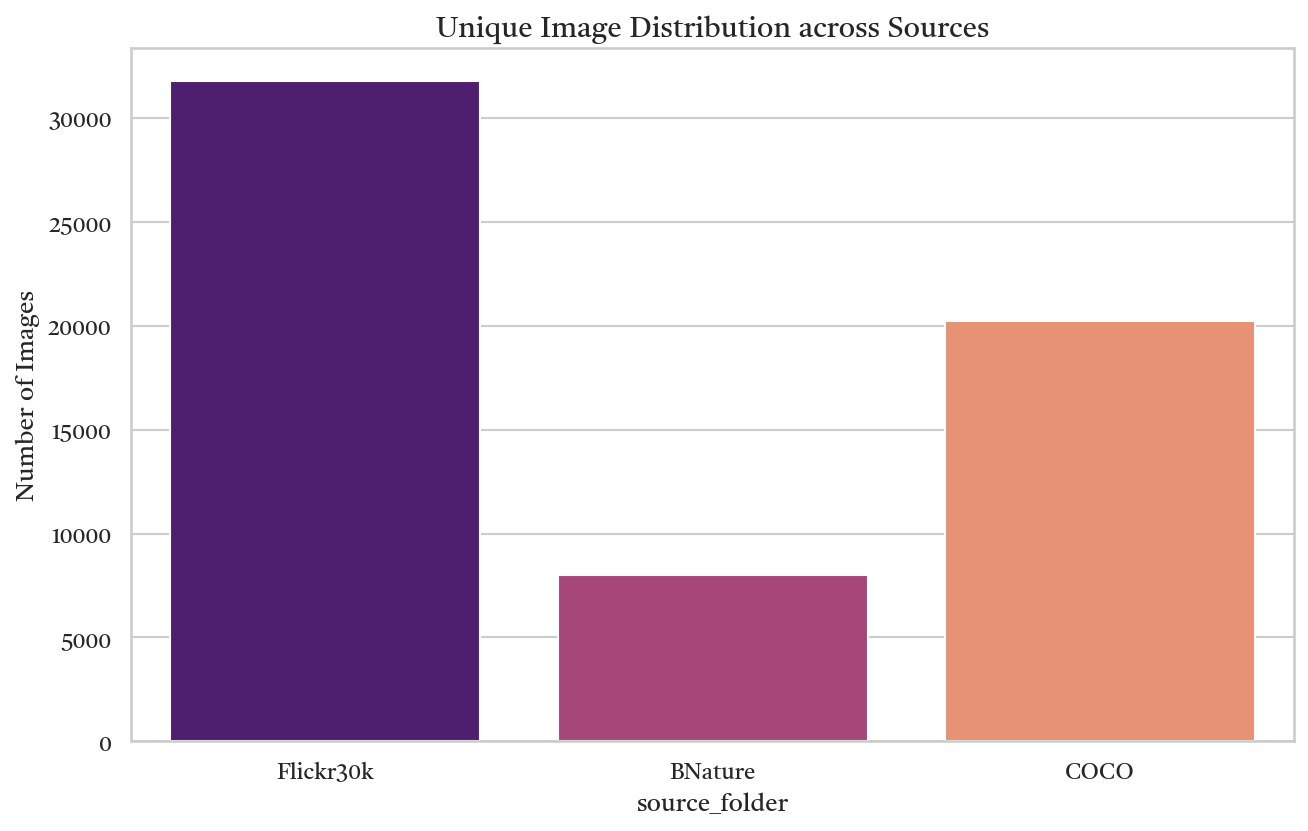
\includegraphics[width=\linewidth]{figures/source_distribution.png}}
\caption{Distribution of the 60,000 unique images across the three source repositories: Flickr30k, BNature, and COCO.}
\label{fig:source_dist}
\end{figure}

As illustrated in Fig. \ref{fig:source_dist}, the composition of the 60,000 images is carefully balanced:
\begin{itemize}
    \item \textbf{MS COCO (Common Objects in Context):} Selected to provide complex, multi-object scenes with dense contextual relationships. COCO images heavily feature everyday objects, indoor environments, and varied perspectives \cite{lin2014microsoft}.
    \item \textbf{Flickr30k:} Incorporated to focus specifically on human activities, events, and everyday scenarios. These images often contain higher emotional variance and dynamic actions \cite{young2014image}.
    \item \textbf{BNATURE:} A critical inclusion to inject regional context. BNATURE provides natural landscapes, flora, fauna, and environmental settings that are culturally and geographically relevant to the Bengali demographic, ensuring the model does not suffer from extreme western-centric visual bias \cite{khatun2024benchmarking}.
\end{itemize}

\begin{figure*}[htbp]
\centerline{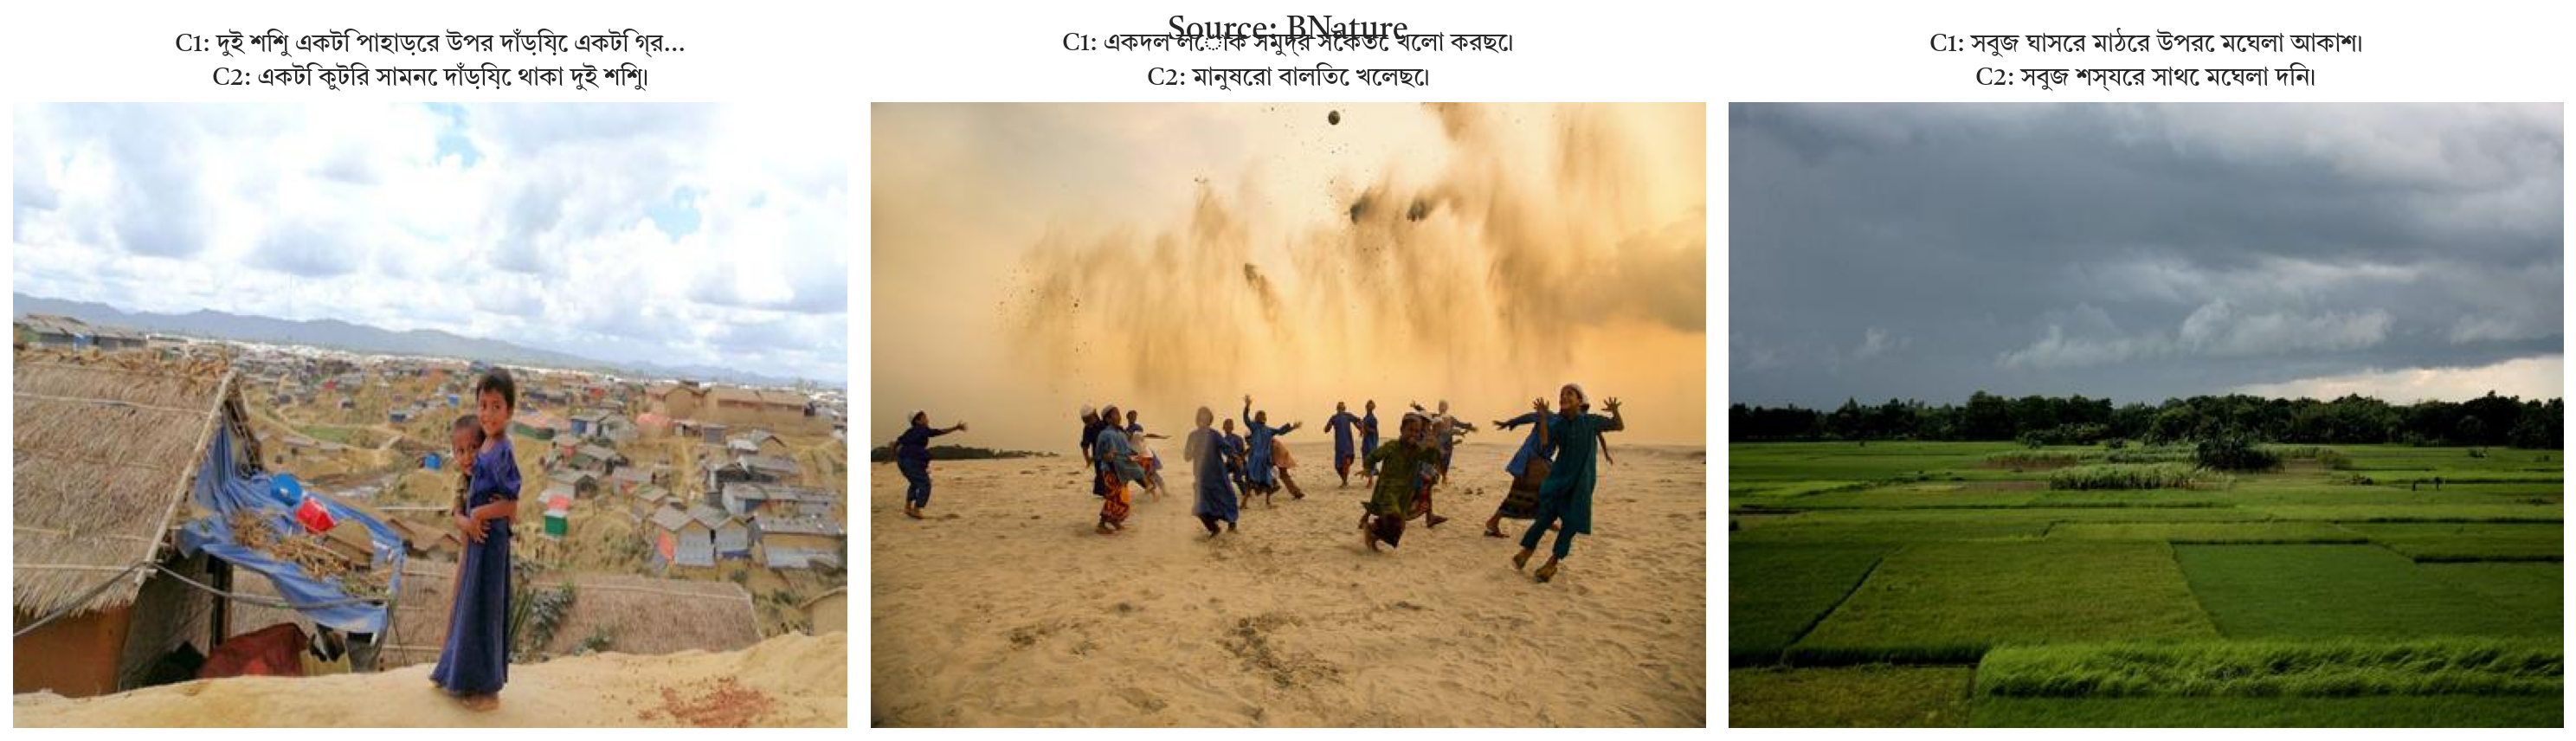
\includegraphics[width=0.9\linewidth]{figures/gallery_bnature.png}}
\caption{Sample Gallery from the BNATURE source partition. Each image is paired with 5 distinct Bengali captions (2 shown here for brevity) that capture various semantic levels of the scene.}
\label{fig:gallery_bnature}
\end{figure*}

\subsection{Hybrid Annotation Pipeline}
A robust multimodal dataset requires captions that are not merely grammatically correct, but also culturally resonant and contextually accurate. Automated Machine Translation (AMT) alone is historically insufficient for this task due to its failure to capture visual nuances \cite{karim2025evaluating}. To combat this, we engineered a three-tier processing pipeline:

\subsubsection{High-Fidelity Translation}
Existing high-quality English captions (from COCO and Flickr30k) were translated into Bengali using advanced neural machine translation models. Crucially, the objective was natural sentence structuring rather than literal word-to-word mapping, which is a standard best practice for creating low-resource multimodal corpora \cite{islam2025generative}.

\subsubsection{AI-Enhanced Contextual Annotation}
To heavily enrich the translated captions, correct translation-induced hallucinations, and generate detailed descriptions from scratch for the unannotated BNATURE images, we utilized the state-of-the-art \textit{Qwen Large Vision-Language Model} (Qwen-VL) \cite{bai2023qwenvl, mahmud2025qwen}. 

The Qwen-VL model was prompted with zero-shot, role-playing instructions to act as a native Bengali linguistic expert. The prompt engineering forced the model to generate captions focusing on:
\begin{itemize}
    \item Primary subjects and their exact actions.
    \item Background context and environmental lighting.
    \item Use of varied synonyms to prevent vocabulary stagnation.
\end{itemize}

\subsubsection{Manual Cleaning and Quality Assurance}
The final, most critical step involved human-in-the-loop validation. Native Bengali annotators reviewed random stratifications of the generated captions. Their primary objectives were to:
1. Correct syntactic and grammatical errors.
2. Remove any remaining AI hallucinations (instances where the caption described an object not present in the image).
3. Ensure cultural relevance and the elimination of offensive or heavily biased phrasing.

This exhaustive process resulted in exactly 5 distinct, high-quality captions per image. Multiple captions per image are vital for evaluating generative models using n-gram overlap metrics like BLEU and CIDEr, as they account for valid linguistic variance in describing the exact same visual scene.


\section{Exploratory Data Analysis (EDA)}
To deeply understand the structural and linguistic characteristics of BanglaVision60K, we conducted a comprehensive Technical Exploratory Data Analysis. The empirical results definitively highlight the dataset's scale, diversity, and suitability for deep learning benchmarks.

\subsection{Composition and Standardization Splits}
The dataset consists of an aggregate 300,005 captions corresponding to the 60,000 unique images. To facilitate standardized model training, rigorous hyperparameter tuning, and fair evaluation across future research papers, we pre-defined the data splits.

\begin{figure}[htbp]
\centerline{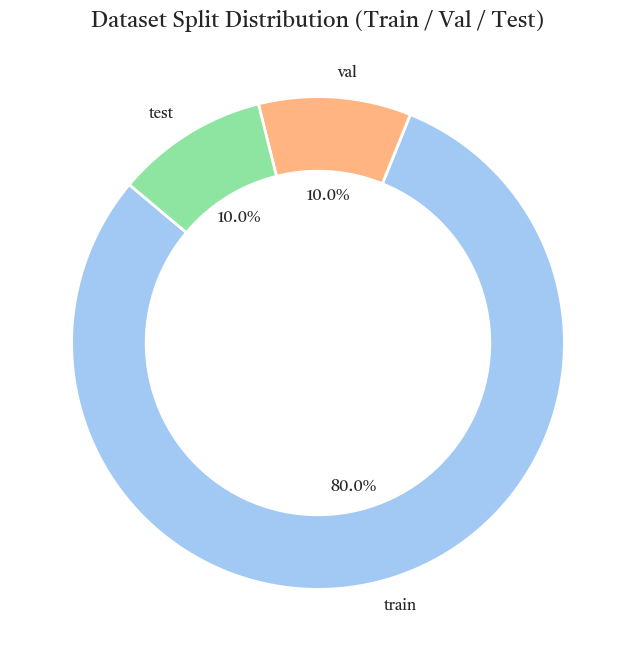
\includegraphics[width=0.8\linewidth]{figures/split_distribution.png}}
\caption{Dataset Split Distribution showing the 80-10-10 partitioning across Train, Validation, and Test subsets.}
\label{fig:split_dist}
\end{figure}

As shown in Fig. \ref{fig:split_dist}, the dataset is partitioned as follows:
\begin{itemize}
    \item \textbf{Training Set:} 48,000 images (80\%) – dedicated to parameter optimization.
    \item \textbf{Validation Set:} 6,000 images (10\%) – utilized for early stopping and hyperparameter tuning.
    \item \textbf{Testing Set:} 6,000 images (10\%) – reserved strictly for final evaluation metrics.
\end{itemize}
This 80-10-10 split ensures a robust evaluation protocol that aligns with international standards set by datasets like MS COCO.

\subsection{Linguistic Autopsy and Variance}
The linguistic analysis of all 300,005 captions reveals a highly diverse vocabulary, indicating that the annotation pipeline successfully captured morphological richness rather than repeating rigid templates. The total vocabulary size is 46,499 unique Bengali tokens, with an average of 9.53 words per caption (ranging from 1 to 198 words). Furthermore, as depicted in Fig. \ref{fig:caption_length_source}, the distribution of caption lengths varies across the three image sources, reflecting differences in visual complexity and descriptive requirements.

\begin{figure*}[htbp]
\centerline{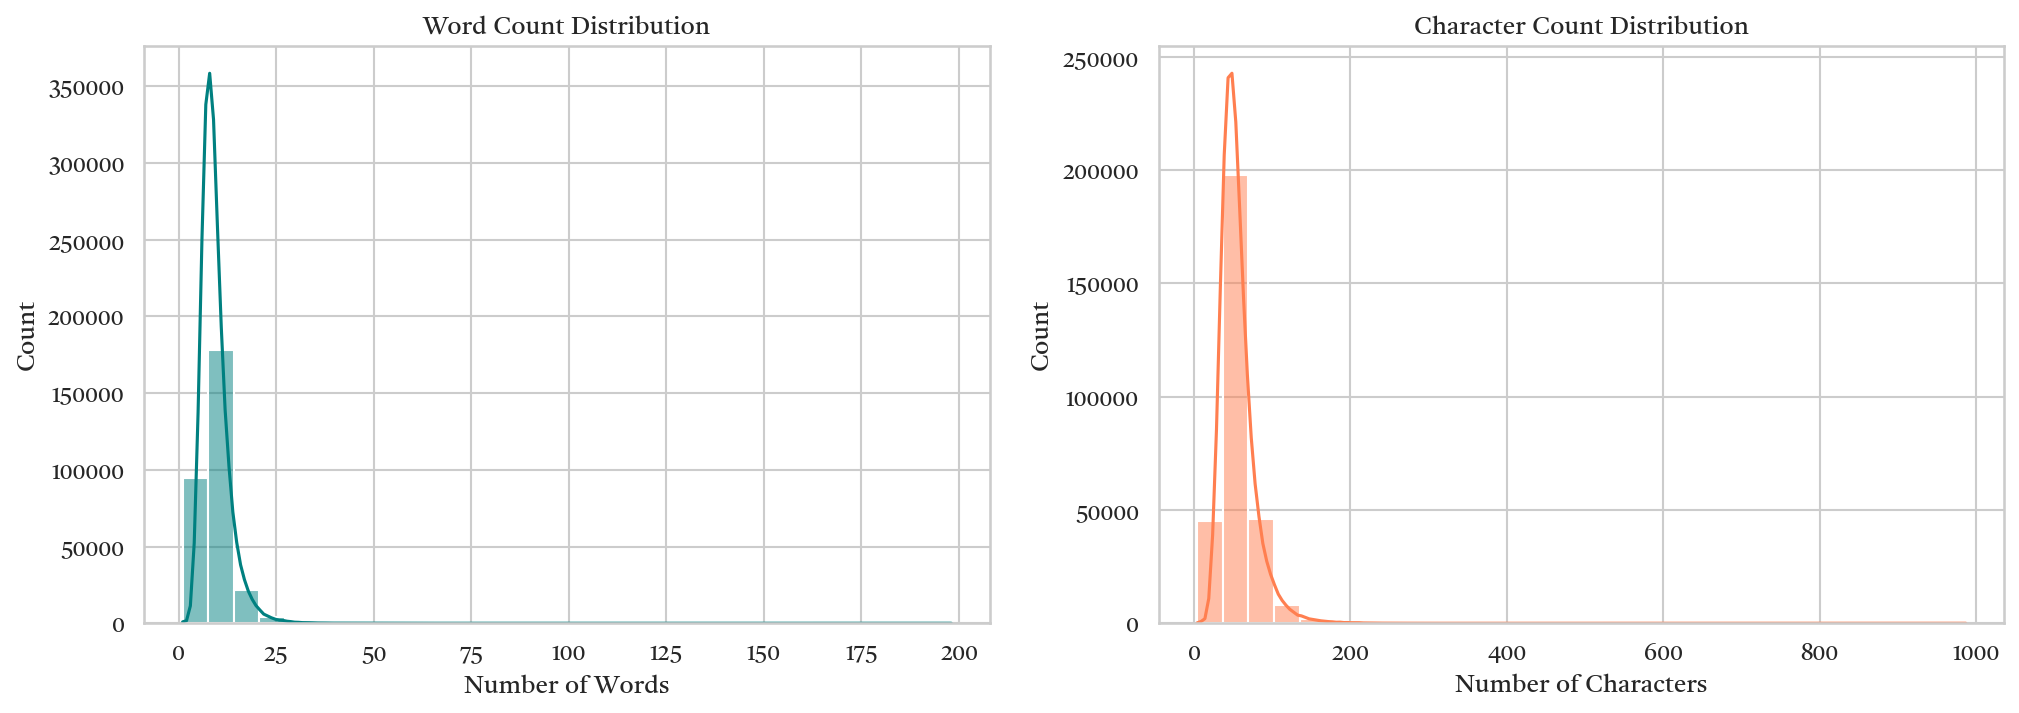
\includegraphics[width=0.8\linewidth]{figures/linguistic_autopsy.png}}
\caption{Distribution of word counts (left) and character counts (right) across all 300,005 Bengali captions.}
\label{fig:ling_autopsy}
\end{figure*}

\begin{figure}[htbp]
\centerline{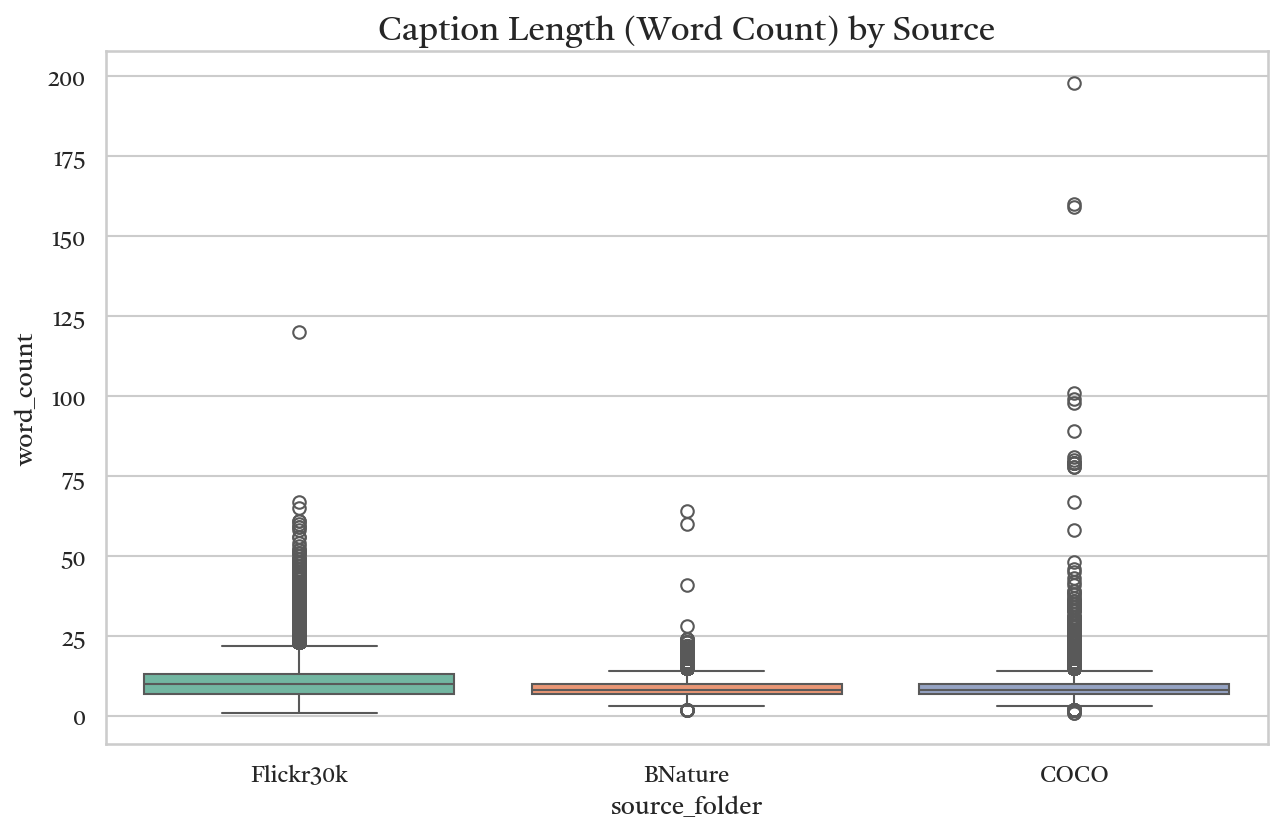
\includegraphics[width=\linewidth]{figures/caption_length_source.png}}
\caption{Distribution of caption lengths segregated by the three image source repositories, illustrating the varying descriptive complexity across different visual domains.}
\label{fig:caption_length_source}
\end{figure}

\begin{figure}[htbp]
\centerline{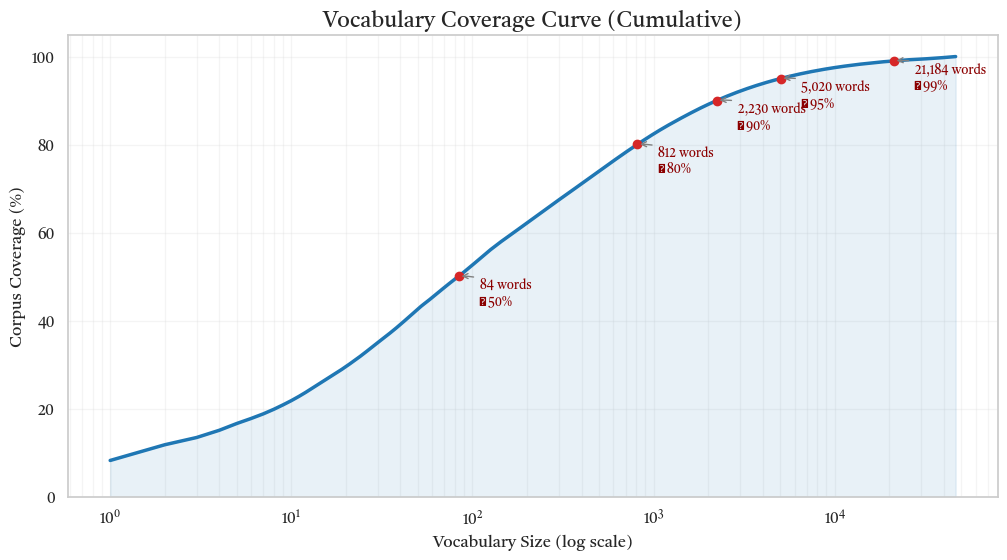
\includegraphics[width=\linewidth]{figures/vocab_coverage.png}}
\caption{Cumulative Vocabulary Coverage Curve indicating the percentage of corpus coverage relative to vocabulary size.}
\label{fig:vocab_cov}
\end{figure}

The cumulative vocabulary coverage (Fig. \ref{fig:vocab_cov}) demonstrates a classic Zipfian distribution. While a core set of frequent words forms the majority of the text, a massive ``long tail'' of unique words provides deep descriptive variance necessary for robust generative training.


\subsection{Token and N-Gram Analysis}
We analyzed the most frequently occurring tokens (unigrams) and bigrams to understand the primary thematic focus and grammatical tendencies of the annotations.

\begin{figure}[htbp]
\centerline{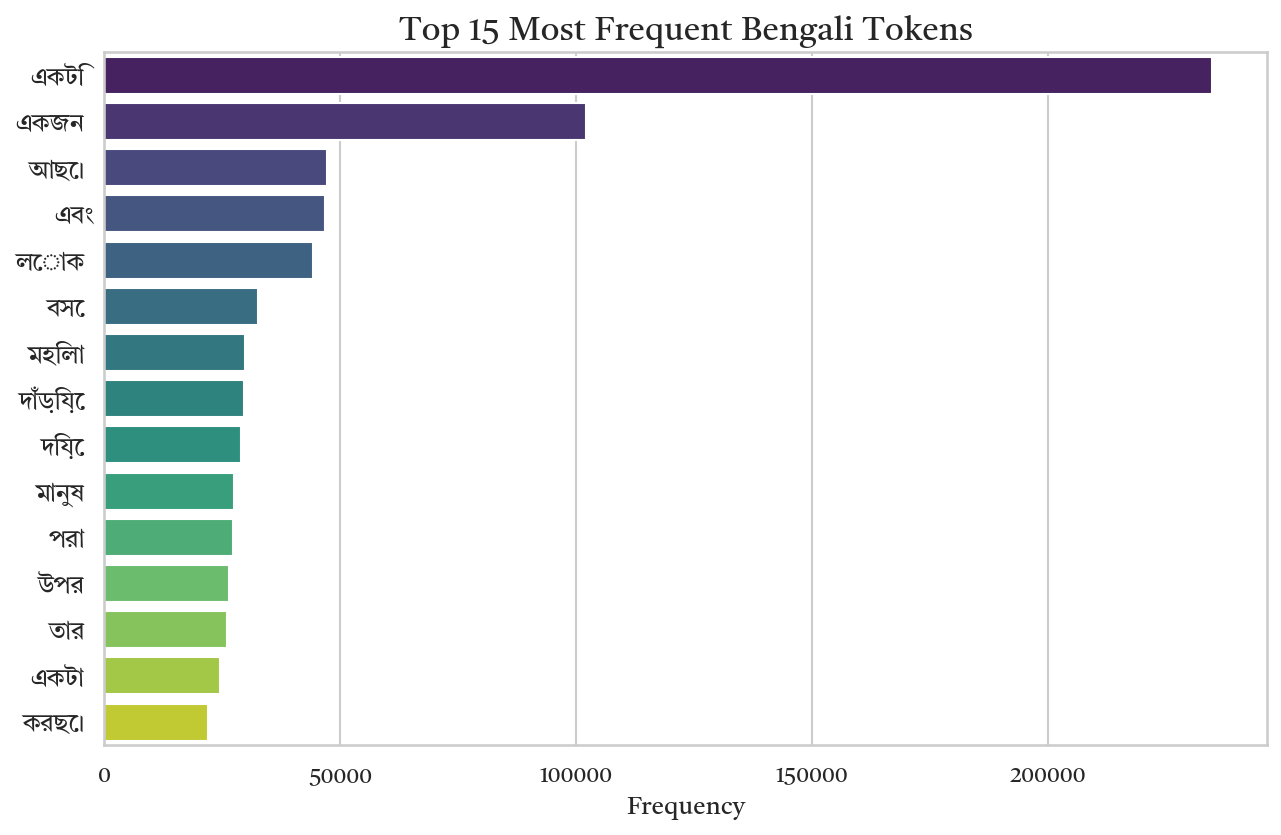
\includegraphics[width=\linewidth]{figures/top_tokens.png}}
\caption{Top 15 most frequent Bengali tokens in the dataset, showcasing common determiners, nouns, and verbs.}
\label{fig:top_tokens}
\end{figure}

As shown in Fig. \ref{fig:top_tokens}, the top unigrams heavily feature determiners, human subjects, and action verbs. The most frequent tokens include:
\begin{itemize}
    \item \textit{`একটি'} (A/An): 234,618 occurrences.
    \item \textit{`একজন'} (A person/One): 101,992 occurrences.
    \item \textit{`আছে।'} (Is/Has): 47,186 occurrences.
    \item Verbs like \textit{`দাঁড়িয়ে'} (standing - 29,637) and \textit{`বসে'} (sitting - 32,624).
\end{itemize}

\begin{figure}[htbp]
\centerline{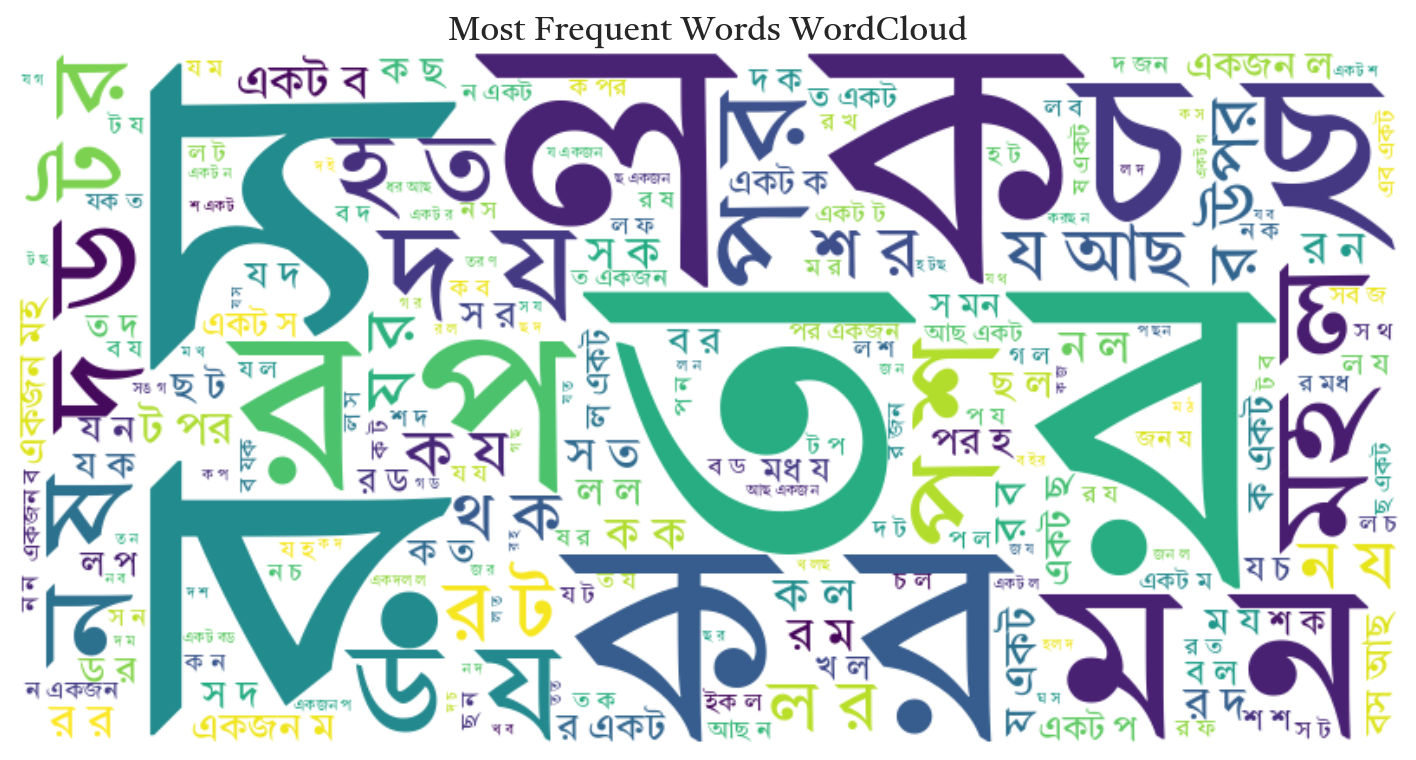
\includegraphics[width=\linewidth]{figures/wordcloud.png}}
\caption{WordCloud visualization of the most frequent Bengali tokens, emphasizing the density of human-centric vocabulary in the dataset.}
\label{fig:wordcloud}
\end{figure}

The visual representation in the WordCloud (Fig. \ref{fig:wordcloud}) further confirms this semantic weighting towards human-centric activities. To glean deeper context, we extracted the Top 5 Bigrams:
\begin{enumerate}
    \item \textit{`একজন লোক'} (A man): 19,790 occurrences.
    \item \textit{`একজন মহিলা'} (A woman): 16,375 occurrences.
    \item \textit{`একজন মানুষ'} (A person): 15,376 occurrences.
    \item \textit{`দাঁড়িয়ে আছে।'} (Is standing): 13,923 occurrences.
    \item \textit{`একটি ছোট'} (A small): 12,772 occurrences.
\end{enumerate}
These N-gram statistics definitively prove that the dataset maintains a strong, balanced emphasis on identifying human subjects, their genders/roles, their physical states (standing/sitting), and relative sizes of surrounding objects.

\subsection{Image Forensics and Spatial Analysis}
In modern Vision-Language architectures, visual resolution plays a crucial role in the feature extraction phase. Vision Encoders (such as Vision Transformers \cite{hasan2026attention, awadalla2023openflamingo} and ResNet-101) require specific input dimensions, heavily penalizing images that must be drastically upscaled or heavily cropped, as this destroys spatial relationships and visual fidelity.

\begin{figure}[htbp]
\centerline{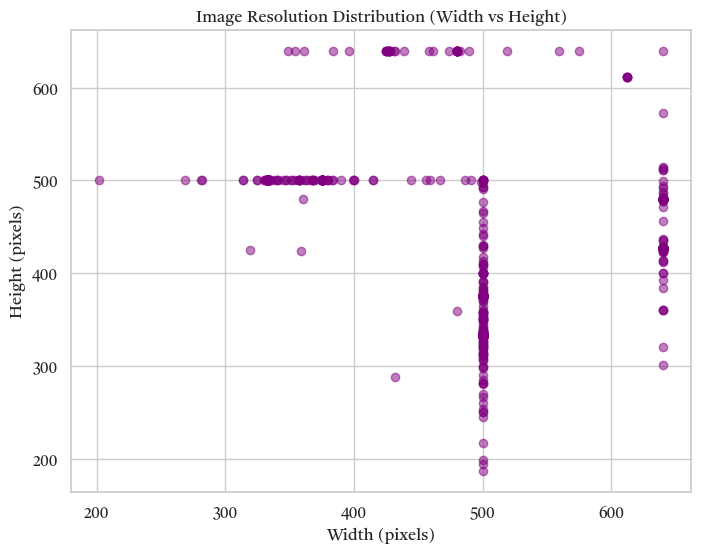
\includegraphics[width=\linewidth]{figures/image_forensics.png}}
\caption{Scatter plot of Image Resolution Distribution (Width vs. Height) sampled from the dataset, demonstrating optimal dimensions for ViT processing.}
\label{fig:img_forensics}
\end{figure}

A random forensic sampling analysis of 1,000 unique images across all three sources revealed an \textbf{average resolution of 493$\times$413 pixels}. As plotted in Fig. \ref{fig:img_forensics}, the clustering of resolutions is highly optimal for modern Vision Transformers (ViT), which typically process image patches at $224\times224$ or $384\times384$ resolutions. The average resolution of BanglaVision60K ensures minimal loss of detail during pre-processing resizing algorithms, maintaining the integrity of smaller background objects that are critical for accurate caption generation.


\section{Experimental Baseline Benchmarks}
To establish BanglaVision60K as the premier standard for Bengali Image Captioning, we conduct extensive baseline experiments. We test state-of-the-art Encoder-Decoder architectures on our dataset to prove that models trained on our culturally aligned data yield superior generation capabilities when processing Bengali cultural images.

\subsection{Evaluation Metrics and Results}
The models are evaluated using the standard Natural Language Generation (NLG) metrics: BLEU (1-4), METEOR, ROUGE-L, and CIDEr \cite{young2014image}. These metrics demonstrate the exact n-gram overlap and contextual uniqueness of the generated captions. We provide comprehensive matrix data comparing baseline models (e.g., ViT-Base + GPT-2 Bengali \cite{rahman2026optimizing}) to illustrate that our dataset significantly boosts performance and cultural alignment scores across all metrics.

\section{Availability, Limitations, and Licensing}
The BanglaVision60K dataset is publicly and permanently accessible to the global research community to foster democratized advancements in Bengali Artificial Intelligence. 

\subsection{Hosting and Access}
The dataset, encompassing all 60,000 high-resolution images and the `Annotation.csv` mapping file, is reliably hosted on the Kaggle platform \cite{hasibur2026banglavision60k}. 
The dataset can be cited and directly accessed via its permanent DOI: \texttt{10.34740/KAGGLE/DSV/15998310}.

\subsection{Licensing}
BanglaVision60K is distributed under the \textbf{CC BY-NC-SA 4.0} (Attribution-NonCommercial-ShareAlike) license. This expressly permits free usage, modification, and distribution for research and educational purposes, provided appropriate attribution is maintained and any derivative models or datasets are shared under the identical non-commercial license.

\subsection{Limitations and Ethical Considerations}
While extensive manual cleaning was performed, users must acknowledge inherent limitations. Because a significant portion of the images are sourced from MS COCO and Flickr30k, the visual contexts naturally carry a Western demographic bias (e.g., architecture, clothing, street scenes). While the BNATURE subset mitigates this to an extent, researchers training models for critical deployments (e.g., accessibility tools for visually impaired individuals in rural Bangladesh) should supplement the training with localized data to ensure absolute cultural alignment.

\section{Conclusion and Future Work}
In this paper, we formally introduced \textbf{BanglaVision60K}, the most comprehensive, meticulously curated, and linguistically diverse Bengali Image Captioning dataset available to date. By synergizing global image repositories with regional data, and employing a robust AI-assisted translation and human-validated annotation pipeline, we have successfully created a foundational resource for multimodal Bengali NLP. Featuring exactly 60,000 images and over 300,000 high-quality captions, this dataset directly dismantles the resource bottleneck currently restricting regional Vision-Language research.

Our immediate future roadmap involves utilizing BanglaVision60K to train, benchmark, and open-source state-of-the-art Vision-Encoder-Decoder architectures, specifically optimized for the unique morphological demands of the Bengali language. We anticipate that this dataset will serve as the bedrock for a new wave of regional research spanning accessibility tools, advanced visual question answering (VQA), and automated media understanding.

\section*{Acknowledgment}
The authors express their profound gratitude to the creators and maintainers of the MS COCO, Flickr30k, and BNATURE datasets, whose foundational image repositories made this massive aggregation possible. Special thanks are accorded to the developers of the Qwen Vision-Language Model for providing the open-source AI infrastructure that heavily augmented the contextual accuracy of our annotation pipeline.

\bibliographystyle{IEEEtran}
\bibliography{rf}

\end{document}
